%%%%%%%%%%%%%%%%%%%%%%%%%%%%%%%%%%%%%%%%%%%%%%%%%%%%%%
% A Beamer template for University of Wollongong     %
% Based on THU beamer theme                          %
% Author: Qiuyu Lu                                   %
% Date: July 2024                                    %
% LPPL Licensed.                                     %
%%%%%%%%%%%%%%%%%%%%%%%%%%%%%%%%%%%%%%%%%%%%%%%%%%%%%%
% Customized for Sharif University of Technology     %
%%%%%%%%%%%%%%%%%%%%%%%%%%%%%%%%%%%%%%%%%%%%%%%%%%%%%%


\documentclass[serif, aspectratio=169]{beamer}
%\documentclass[serif]{beamer}  % for 4:3 ratio
\usepackage[T1]{fontenc} 
\usepackage{fourier} % see "http://faq.ktug.org/wiki/uploads/MathFonts.pdf" for other options
\usepackage{hyperref}
\usepackage{latexsym,amsmath,xcolor,multicol,booktabs,calligra}
\usepackage{graphicx,pstricks,listings,stackengine}
\usepackage{lipsum}
\usepackage{caption}

% For writing clean pseudocodes
\usepackage{algorithm, algpseudocode, mathtools, needspace}
% To justify the items
\usepackage{ragged2e}
% To draw diagrams
\usepackage{tikz}
% To include urls
\usepackage{url}
% To make clean tables
\usepackage{color, tabularray}

\author{Ali Sharifi-Zarchi}
\title{Machine Learning (CE 40717)}
\subtitle{Fall 2024}
\institute{
    CE Department \\
    Sharif University of Technology
}
\usepackage{SUTstyle}

% defs
\def\cmd#1{\texttt{\color{red}\footnotesize $\backslash$#1}}
\def\env#1{\texttt{\color{blue}\footnotesize #1}}
\definecolor{deepblue}{rgb}{0,0,0.5}
\definecolor{deepred}{RGB}{153,0,0}
\definecolor{deepgreen}{rgb}{0,0.5,0}
\definecolor{halfgray}{gray}{0.55}
\definecolor{silver}{rgb}{0.752,0.752,0.752}

\lstset{
    basicstyle=\ttfamily\small,
    keywordstyle=\bfseries\color{deepblue},
    emphstyle=\ttfamily\color{deepred},    % Custom highlighting style
    stringstyle=\color{deepgreen},
    numbers=left,
    numberstyle=\small\color{halfgray},
    rulesepcolor=\color{red!20!green!20!blue!20},
    frame=shadowbox,
}



\begin{document}

\begin{frame}
    \titlepage
    \vspace*{-0.6cm}
    \begin{figure}[htpb]
        \begin{center}
            
\includegraphics[keepaspectratio, scale=0.25]{pic/sharif-main-logo.png}
        \end{center}
    \end{figure}
\end{frame}

\begin{frame}    
\tableofcontents[sectionstyle=show,
subsectionstyle=show/shaded/hide,
subsubsectionstyle=show/shaded/hide]
\end{frame}



\section{Introduction}


% Slide 1: Introduction to NLP and Language Importance
\begin{frame}{Natural Language Processing}
	\begin{itemize}
		\item Language is central to human interaction; many of our daily activities revolve around text and language.
		\item Natural Language Processing (NLP) enables computers to understand and generate human language.
	\end{itemize}
\end{frame}

% Slide 2: Translation
\begin{frame}{Translation}
	\begin{figure}
		\centering
		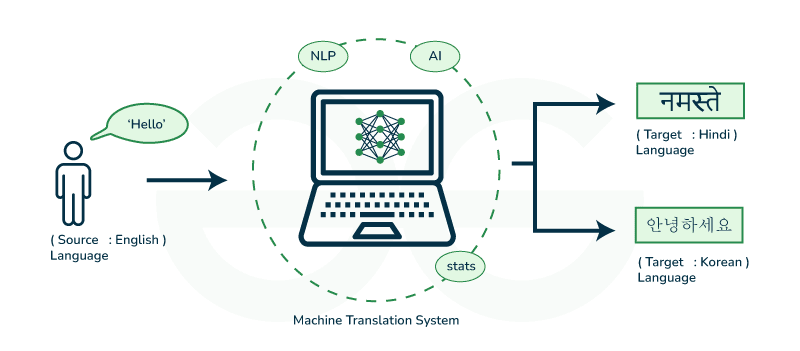
\includegraphics[width=0.6\textwidth]{pic/translation_image.png}
	\end{figure}
	\begin{itemize}
		\item NLP helps translate text from one language to another.
	\end{itemize}
	\vspace{1.6cm}
	\hspace{-1.0cm}
	{\tiny \textcolor{gray}{Figure adapted from geeksforgeeks.org/machine-translation-of-languages-in-artificial-intelligence/}}
\end{frame}

% Slide 3: Sentiment Analysis
\begin{frame}{Sentiment Analysis}
	\begin{figure}
		\centering
		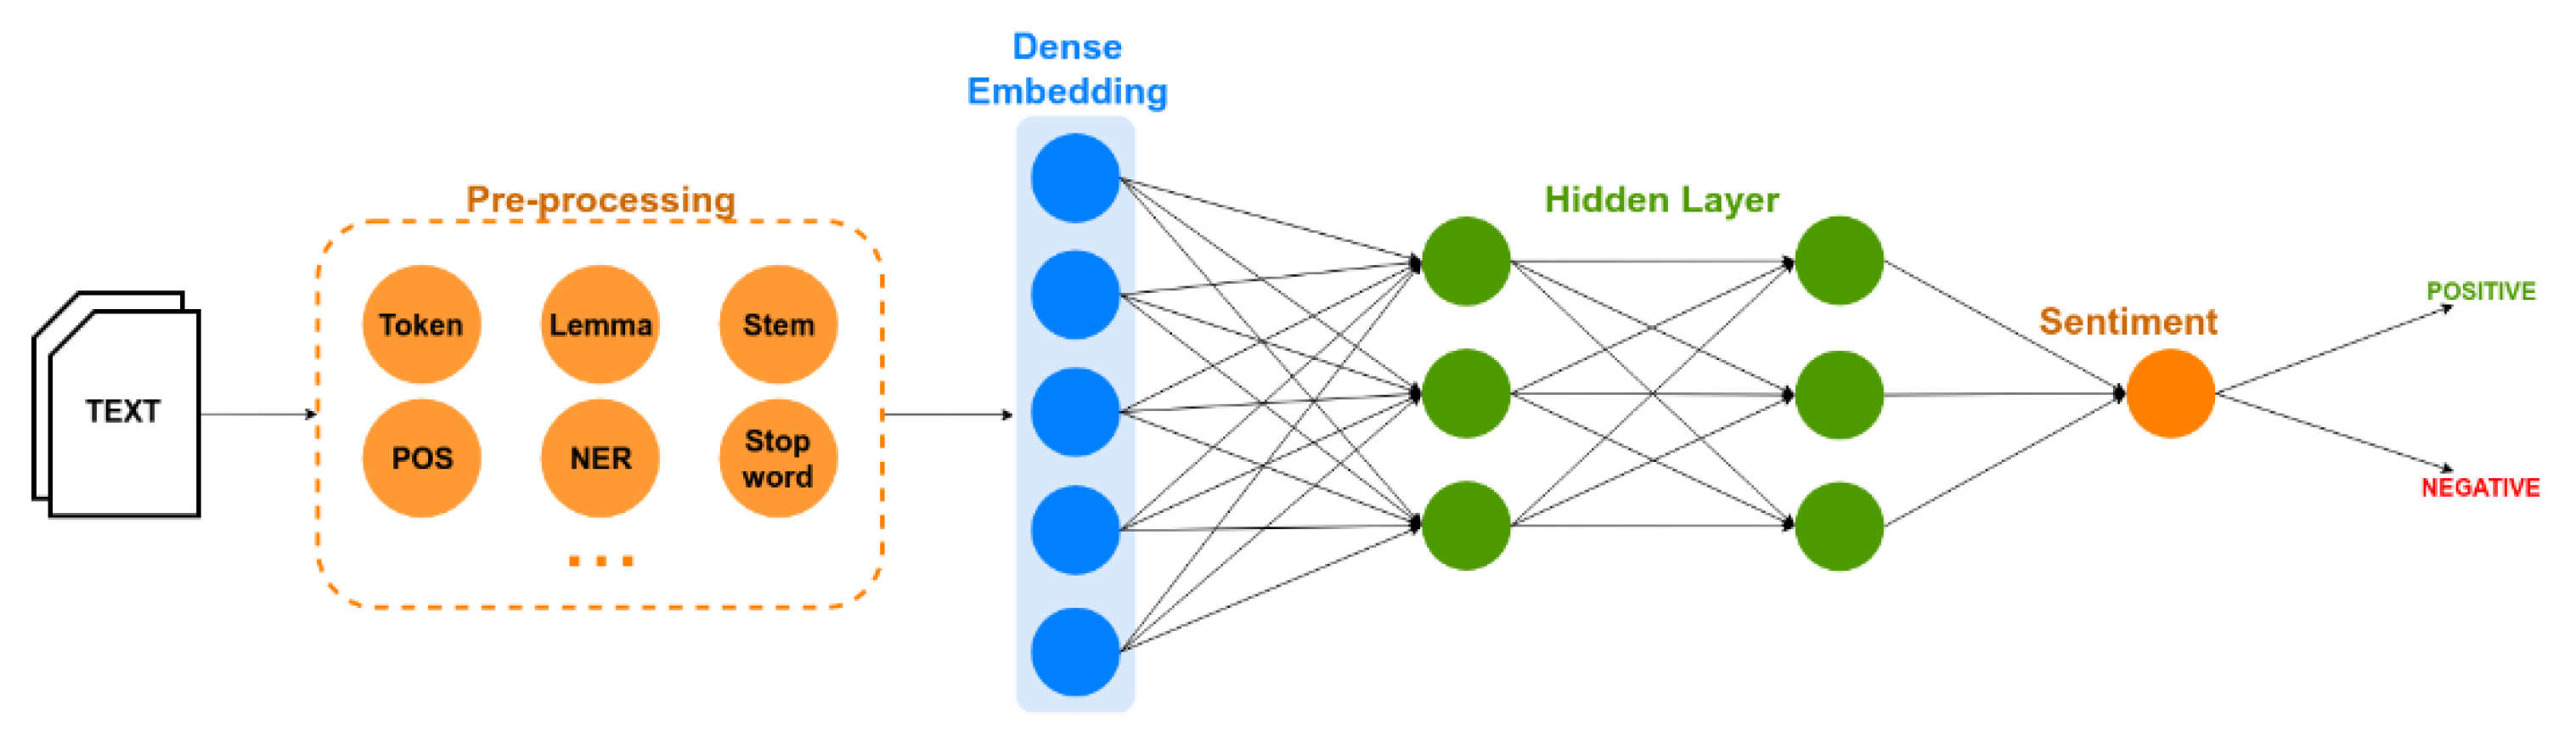
\includegraphics[width=0.6\textwidth]{pic/5.png}
	\end{figure}
	\begin{itemize}
		\item Determines the sentiment (e.g., positive or negative) expressed in a text.
	\end{itemize}
	\vspace{2.6cm}
	\hspace{-1.0cm}
	{\tiny \textcolor{gray}{Figure adapted from www.mdpi.com/2079-9292/9/3/483}}
\end{frame}

% Slide 4: Text Summarization
\begin{frame}{Text Summarization}
	\begin{figure}
		\centering
		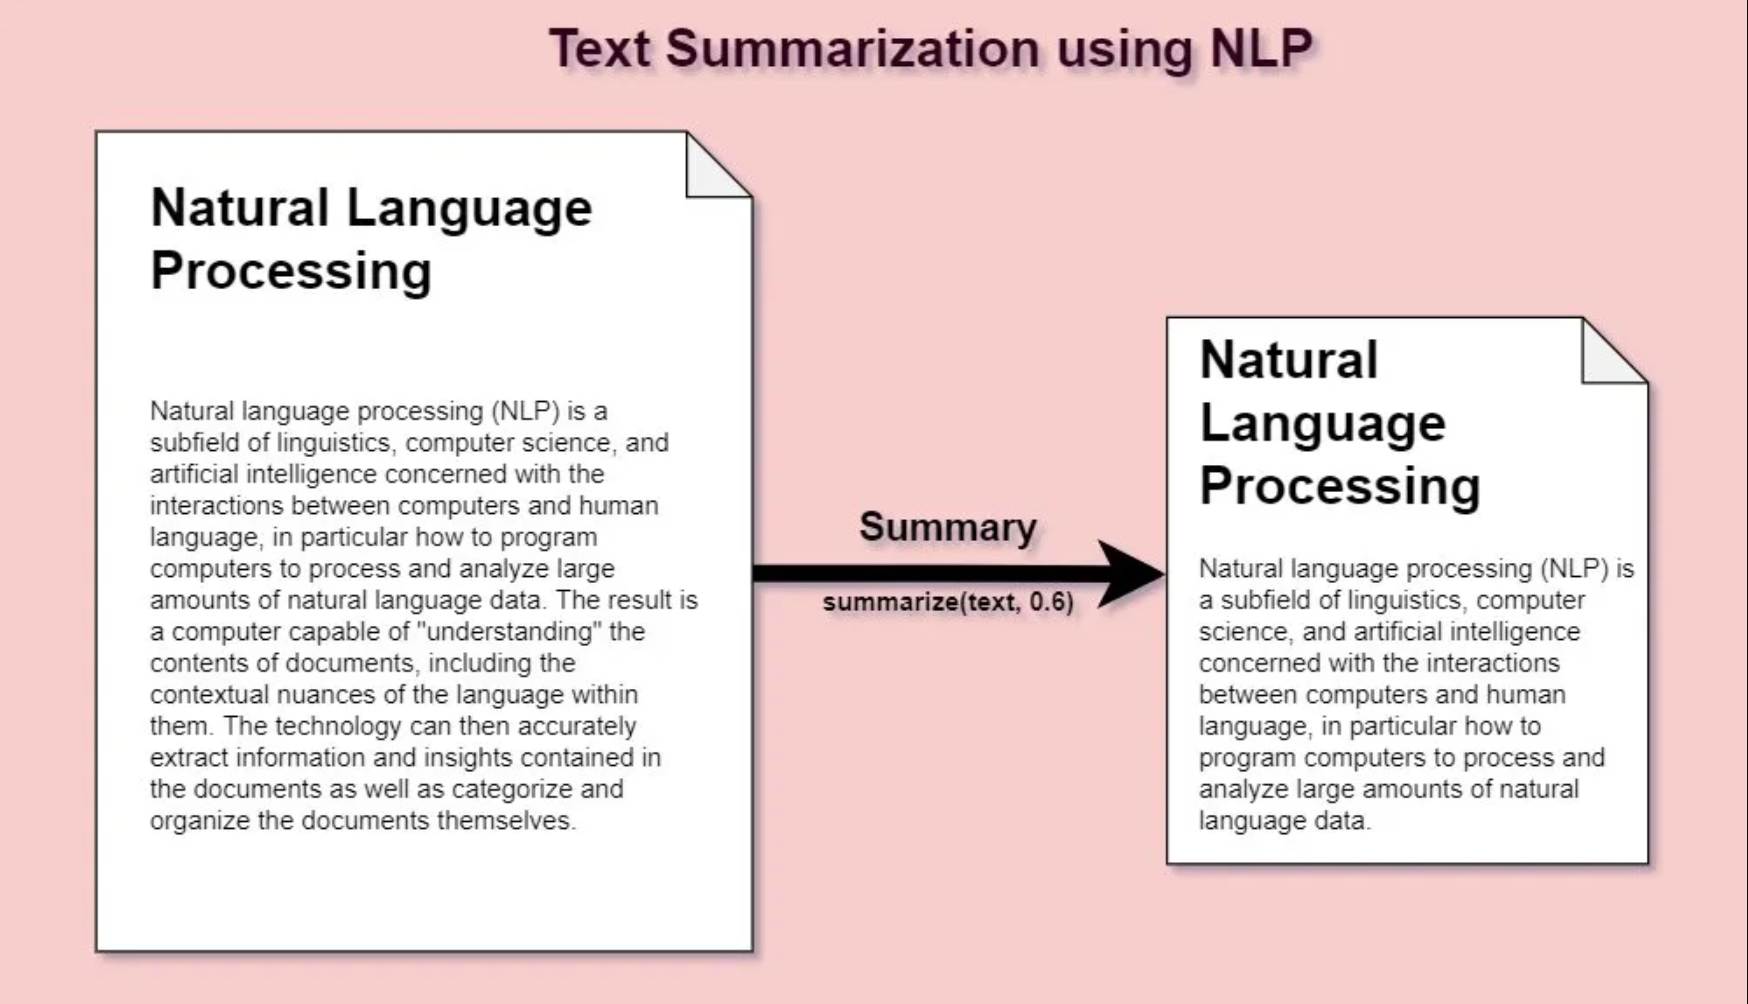
\includegraphics[width=0.6\textwidth]{pic/summarization_image.png}
	\end{figure}
	\begin{itemize}
		\item Automatically generates a concise summary of longer text.
	\end{itemize}
	\vspace{0.6cm}
	\hspace{-1.0cm}
	{\tiny \textcolor{gray}{Figure adapted from turbolab.in/types-of-text-summarization-extractive-and-abstractive-summarization-basics/}}
\end{frame}

% Slide 5: Named Entity Recognition (NER)
\begin{frame}{Named Entity Recognition (NER)}
	\begin{figure}
		\centering
		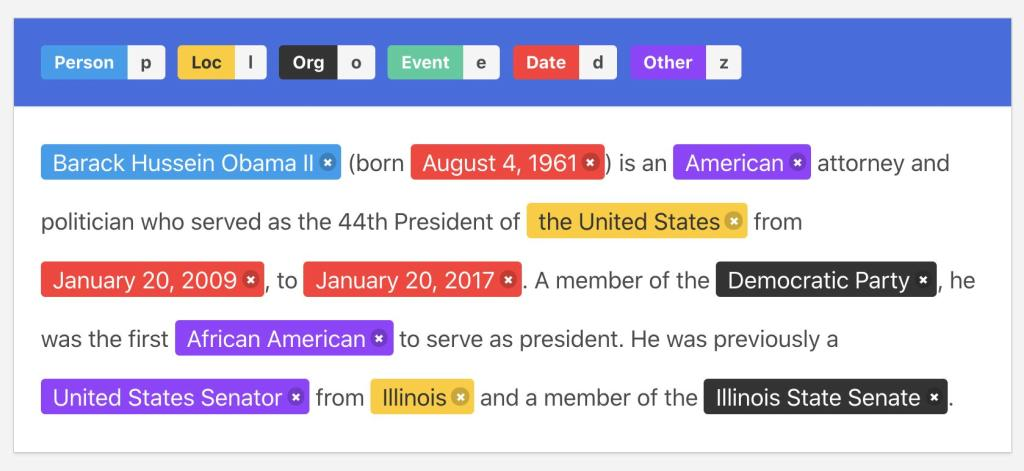
\includegraphics[width=0.6\textwidth]{pic/ner_image.jpg}
	\end{figure}
	\begin{itemize}
		\item Identifies and classifies entities (e.g., names, dates) in text.
	\end{itemize}
	\vspace{1.6cm}
	\hspace{-1.0cm}
	{\tiny \textcolor{gray}{Figure adapted from analyticsvidhya.com/blog/2021/11/a-beginners-introduction-to-ner-named-entity-recognition/}}
\end{frame}

% Slide 6: Speech Recognition
\begin{frame}{Speech Recognition}
	\begin{figure}
		\centering
		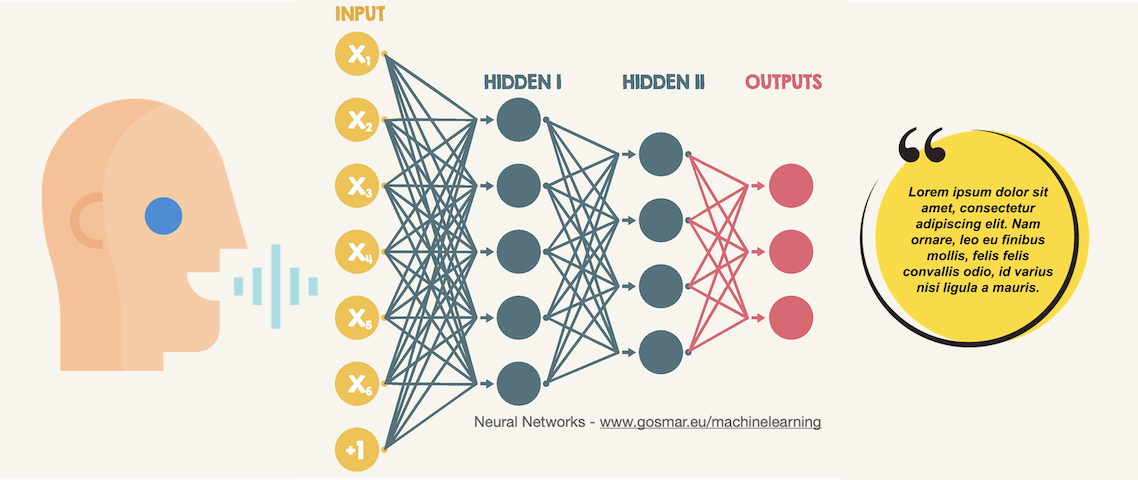
\includegraphics[width=0.6\textwidth]{pic/speech_recognition_image.png}
	\end{figure}
	\begin{itemize}
		\item Converts spoken language into text.
	\end{itemize}
\end{frame}

% Slide 7: Text Classification
\begin{frame}{Text Classification}
	\begin{figure}
		\centering
		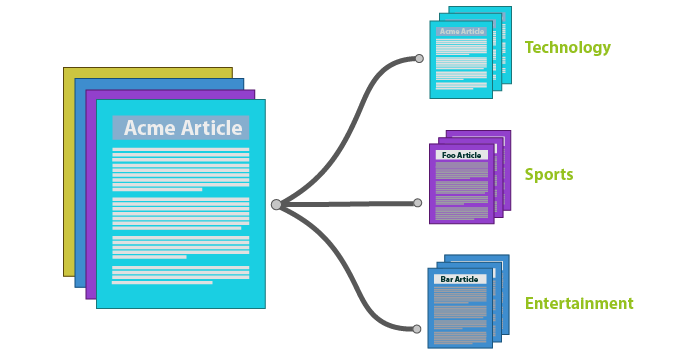
\includegraphics[width=0.6\textwidth]{pic/classification_image.png}
	\end{figure}
	\begin{itemize}
		\item Categorizes text into predefined groups or topics.
	\end{itemize}
	\vspace{1.6cm}
	\hspace{-1.0cm}
	{\tiny \textcolor{gray}{Figure adapted from towardsdatascience.com/machine-learning-nlp-text-classification-using-scikit-learn-python-and-nltk-c52b92a7c73a}}
\end{frame}

% Slide 8: Question Answering
\begin{frame}{Question Answering}
	\begin{figure}
		\centering
		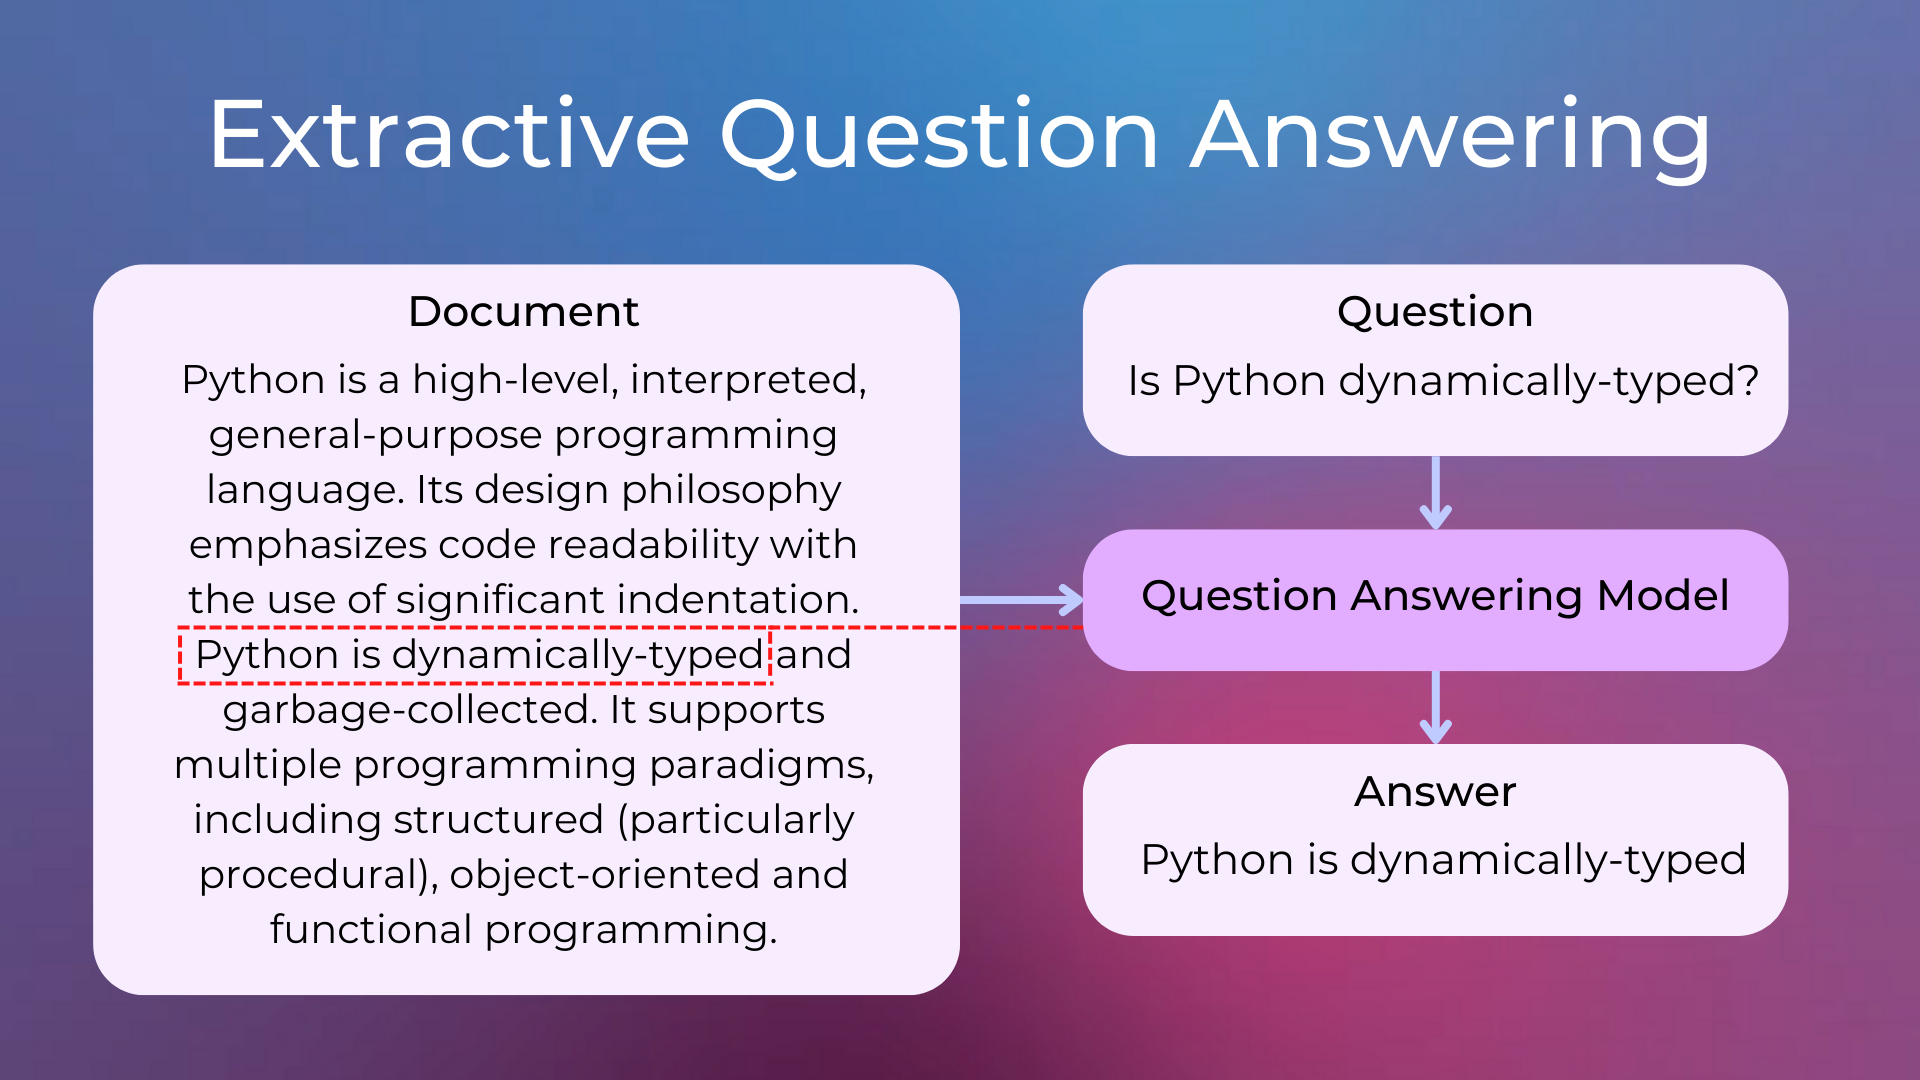
\includegraphics[width=0.6\textwidth]{pic/question_answering_image.png}
	\end{figure}
	\begin{itemize}
		\item Answers questions based on a given text or dataset.
	\end{itemize}
	\vspace{0.6cm}
	\hspace{-1.0cm}
	{\tiny \textcolor{gray}{Figure adapted from nlplanet.org/course-practical-nlp/02-practical-nlp-first-tasks/17-question-answering}}
\end{frame}

% Slide 9: Chatbots and Dialogue Systems
\begin{frame}{Chatbots and Dialogue Systems}
	\begin{figure}
		\centering
		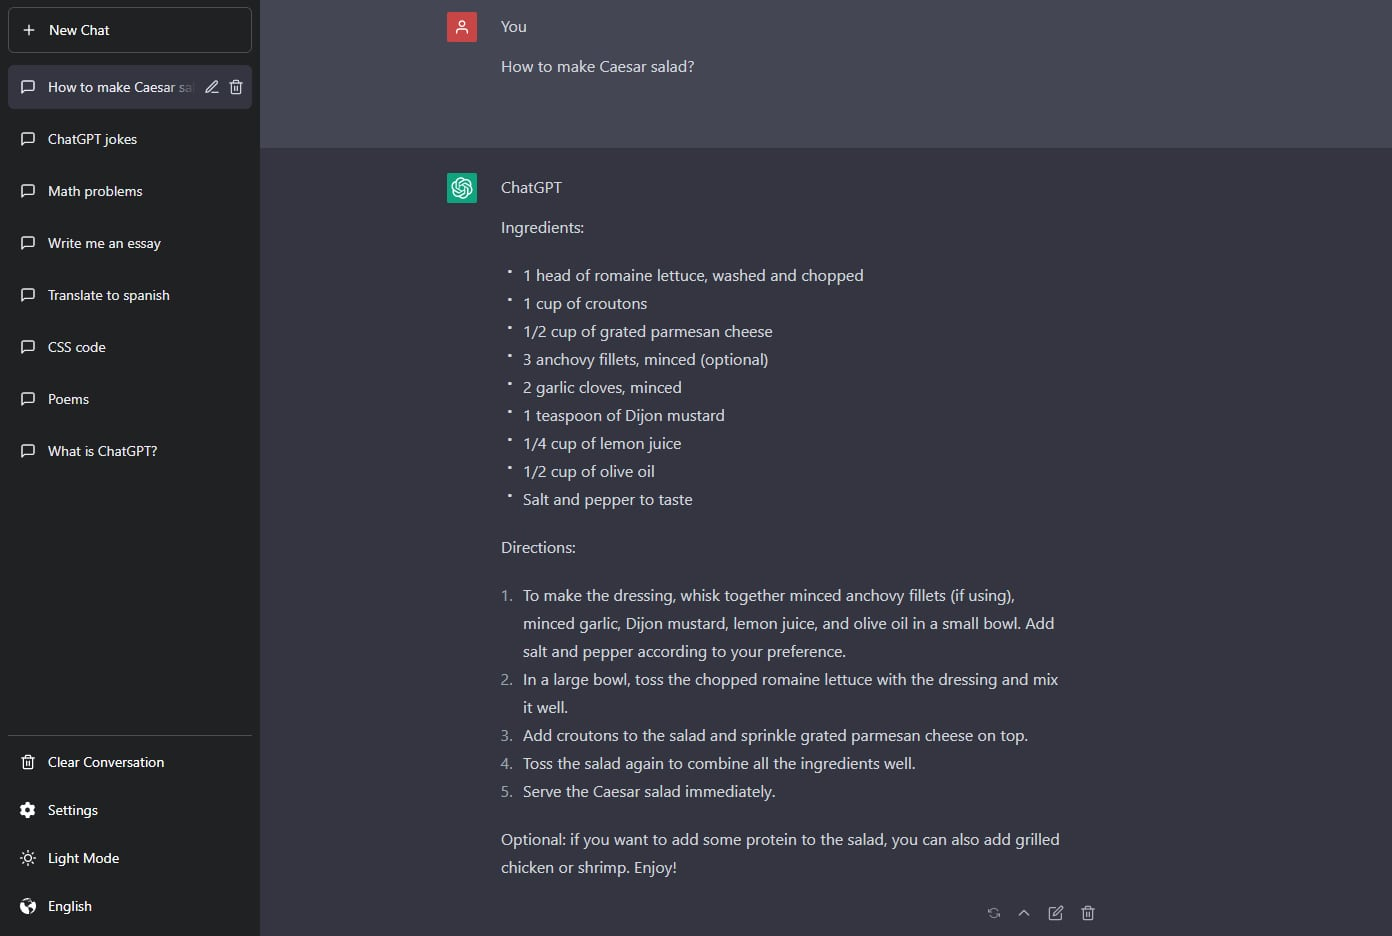
\includegraphics[width=0.6\textwidth]{pic/chatbot_image.jpg}
	\end{figure}
	\begin{itemize}
		\item NLP powers chatbots that can interact with users through text or speech.
	\end{itemize}
	\vspace{0.3cm}
	\hspace{-1.0cm}
	{\tiny \textcolor{gray}{Figure adapted from chatgpt.org/}}
\end{frame}

%% Slide 10: Text Generation
%\begin{frame}{Text Generation}
%	\begin{figure}
%		\centering
%		\includegraphics[width=0.6\textwidth]{pic/text_generation_image.png}
%	\end{figure}
%	\begin{itemize}
%		\item Generates text content, such as stories or articles, from scratch.
%	\end{itemize}
%	\vspace{1.6cm}
%	\hspace{-1.0cm}
%	{\tiny \textcolor{gray}{Figure adapted from www.mdpi.com/2079-9292/9/3/483}}
%\end{frame}

% Slide 11: Transition to Word Representation
\begin{frame}{The Importance of Word Representation}
	\begin{itemize}
		\item To process text effectively, the first step is to represent words in a way that models can understand.
		\item We need to transform words into vectors or dense representations to capture their meaning and relationships.
		\item This is crucial for enabling machines to understand and use language as humans do.
	\end{itemize}
\end{frame}



\begin{frame}{Motivation}
    \begin{itemize}
        \item Traditional models use methods like one-hot encoding, which lacks semantic understanding and cannot capture relationships between words.
        \item We need better word representations that are both dense and semantic.
    \end{itemize}
\end{frame}



\begin{frame}{Definition of One-Hot Encoding}
	\begin{itemize}
		\item One-hot encoding is a straightforward method for representing categorical data, such as words, as discrete vectors.
		\item Each word is represented as a binary vector with the same length as the vocabulary size.
		\item All vector elements are set to 0 except for one position, which is set to 1, identifying the word's unique position in the vocabulary.
	\end{itemize}
\end{frame}

\begin{frame}{Example of One-Hot Encoding}
	\begin{itemize}
		\item For example, given a vocabulary of 5 words:
		\begin{itemize}
			\item \texttt{apple} = [1, 0, 0, 0, 0]
			\item \texttt{banana} = [0, 1, 0, 0, 0]
			\item \texttt{cherry} = [0, 0, 1, 0, 0]
			\item \texttt{date} = [0, 0, 0, 1, 0]
			\item \texttt{elderberry} = [0, 0, 0, 0, 1]
		\end{itemize}
		\item The length of the one-hot vector depends on the number of unique words in the vocabulary.
	\end{itemize}
\end{frame}

\begin{frame}{Strengths and Limitations of One-Hot Encoding}
	\begin{itemize}
		\item \textbf{Strengths:}
		\begin{itemize}
			\item One-hot encoding is a simple and intuitive representation that can be effective in certain models, especially smaller neural networks.
			\item It requires minimal computation and works well for small vocabularies or categorical features in simpler tasks.
		\end{itemize}
		\item \textbf{Limitations:}
		\begin{itemize}
			\item One-hot encoding does not capture any semantic relationships between words.
			\item The vectors are sparse, containing mostly zeros, which is inefficient for large vocabularies.
			\item Similar words (like \texttt{hotel} and \texttt{motel}) appear completely unrelated in this representation.
		\end{itemize}
	\end{itemize}
\end{frame}

\begin{frame}{Example: Similar Words, 0 Cosine Similarity}
	\begin{itemize}
		\item Consider the following one-hot vectors:
		\begin{itemize}
			\item \texttt{hotel} = [0, 0, 0, 1, 0]
			\item \texttt{motel} = [0, 0, 0, 0, 1]
		\end{itemize}
		\item Even though \texttt{hotel} and \texttt{motel} are semantically similar, their cosine similarity is 0 because their vectors are orthogonal.
		\item \textbf{Cosine Similarity:}
		\[
		\cos(\theta) = \frac{\mathbf{v}_1 \cdot \mathbf{v}_2}{\|\mathbf{v}_1\| \|\mathbf{v}_2\|}
		\]
		\item In this case, the dot product of the one-hot vectors is zero, leading to a cosine similarity of zero.
	\end{itemize}
\end{frame}

\begin{frame}{Conclusion: Why Move Beyond One-Hot?}
	\begin{itemize}
		\item While one-hot encoding is a simple and effective method for certain applications, it fails to capture word meanings or relationships.
		\item More advanced methods, such as word embeddings, address these limitations by representing words in a dense, meaningful vector space.
	\end{itemize}
\end{frame}


%\begin{frame}{Word Embedding and Semantic Analysis}
%    \begin{itemize}
%        \item \textbf{Word Embedding:} Represents words as dense vectors in a continuous space, allowing similar words to be mapped close to each other.
%        \item \textbf{Semantic Analysis:} By capturing the context of words, word embeddings enable better performance in tasks like sentiment analysis.
%    \end{itemize}
%\end{frame}

%\begin{frame}{Sentiment Analysis with Word Embeddings}
%    \begin{itemize}
%        \item Sentiment analysis determines the sentiment (e.g., positive or negative) expressed in text.
%        \item Word embeddings capture word context, helping models understand phrases like "not bad" as positive, improving sentiment analysis accuracy.
%    \end{itemize}
%\end{frame}

%\begin{frame}{Sentiment Analysis Pipeline}
%    
%    \begin{figure}
%        \centering
%        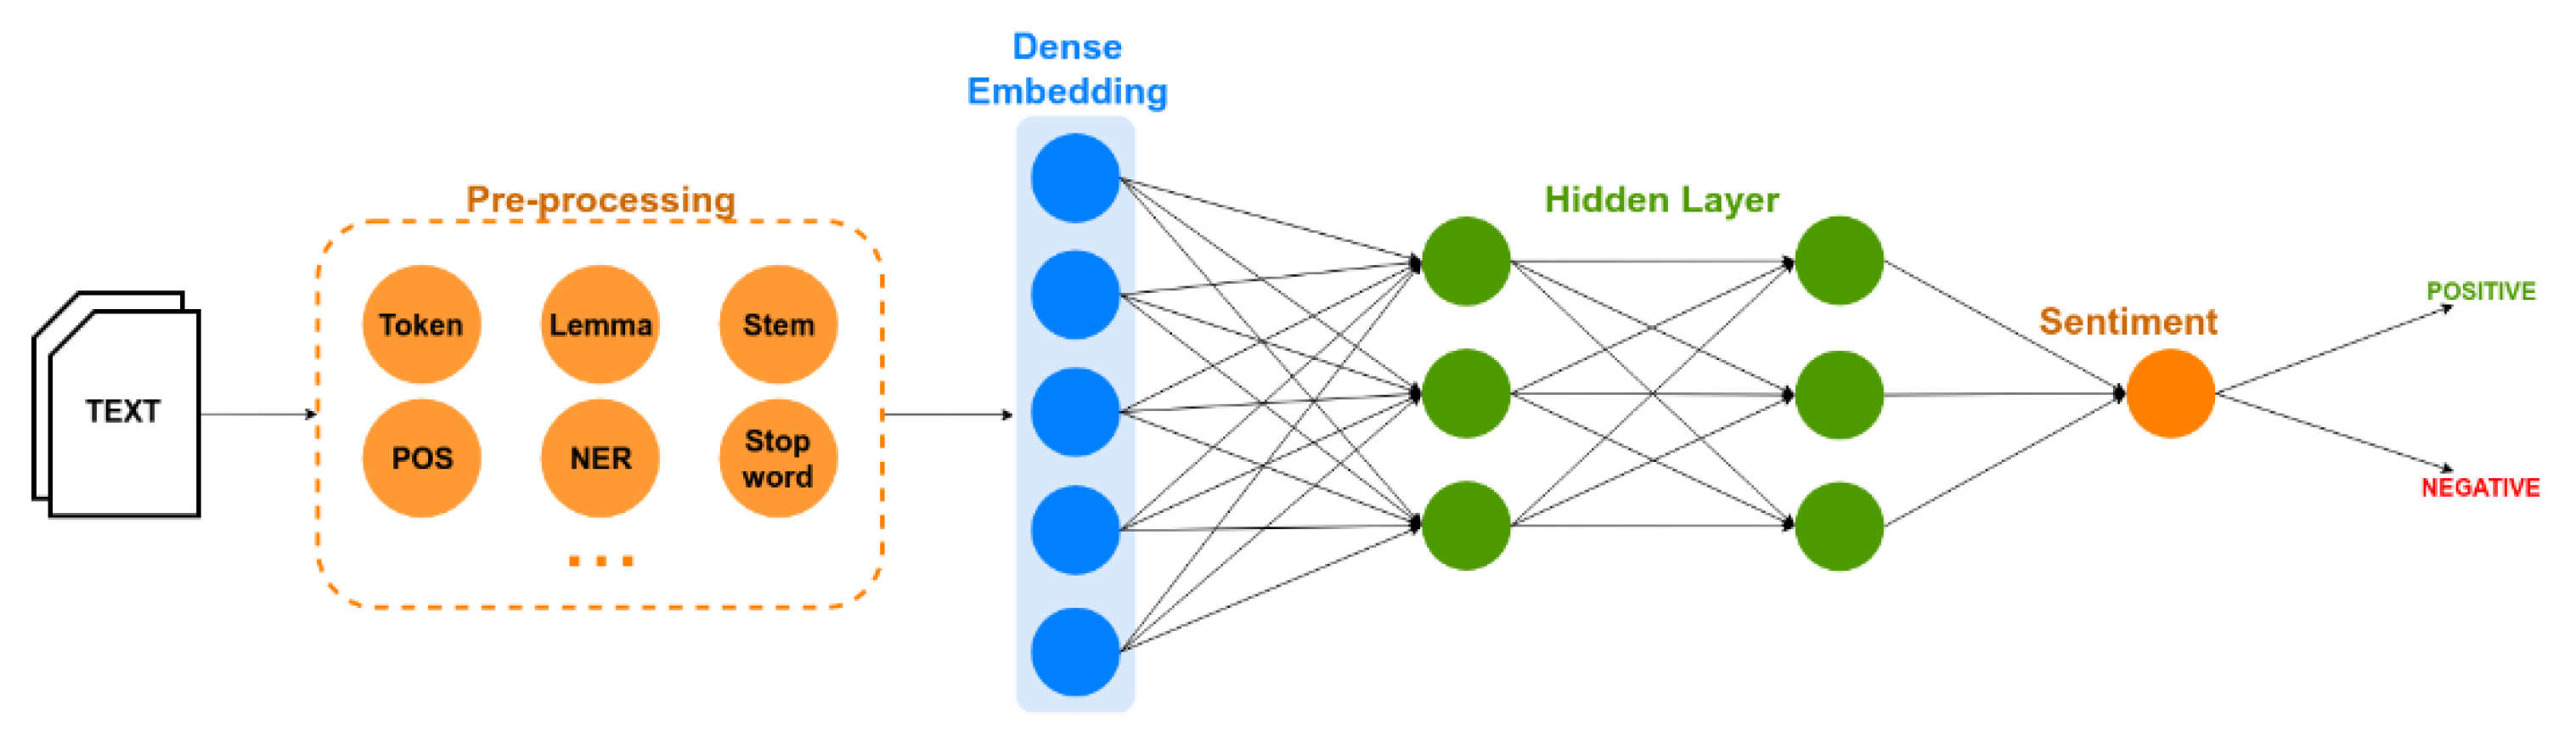
\includegraphics[width=0.6\textwidth]{pic/5.png}
%        \caption*{Sentiment analysis process using word representations}
%    \end{figure}
%    \begin{itemize}
%        \item The process typically involves extracting features (word embeddings), feeding them into a classifier, and predicting the sentiment of the input text.
%    \end{itemize}
%    \vspace{1.6cm}
%    \hspace{-1.0cm}
%    {\tiny \textcolor{gray}{Figure adapted from www.mdpi.com/2079-9292/9/3/483}}
%\end{frame}
%

%
%
%
%
%\section{Latent Semantic Indexing (LSI)}
%
%\begin{frame}{What is Latent Semantic Indexing (LSI)?}
%    \begin{itemize}
%        \item LSI is a technique that decomposes the document-term matrix into a lower-dimensional space.
%        \item By reducing the dimensionality of this matrix, LSI preserves the most significant information while eliminating noise.
%        \item This decomposition helps capture semantic relationships between words and documents, making it valuable for understanding underlying patterns.
%    \end{itemize}
%\end{frame}
%
%\begin{frame}{How Does LSI Work?}
%    \begin{itemize}
%        \item LSI utilizes Singular Value Decomposition (SVD) to factorize the document-term matrix into three matrices:
%        \begin{itemize}
%            \item \( U \): A matrix where each column represents a word in the new, reduced-dimensional space.
%            \item \( \Sigma \): A diagonal matrix of singular values that ranks the importance of each dimension.
%            \item \( V^\top \): A matrix where each row represents a document in the reduced space.
%        \end{itemize}
%        \item By keeping only the top \( k \) singular values, we reduce the matrix to a \( k \)-dimensional space.
%    \end{itemize}
%\end{frame}
%
%\begin{frame}{LSI Example: Document-Term Matrix Decomposition}
%    \begin{figure}
%        \centering
%        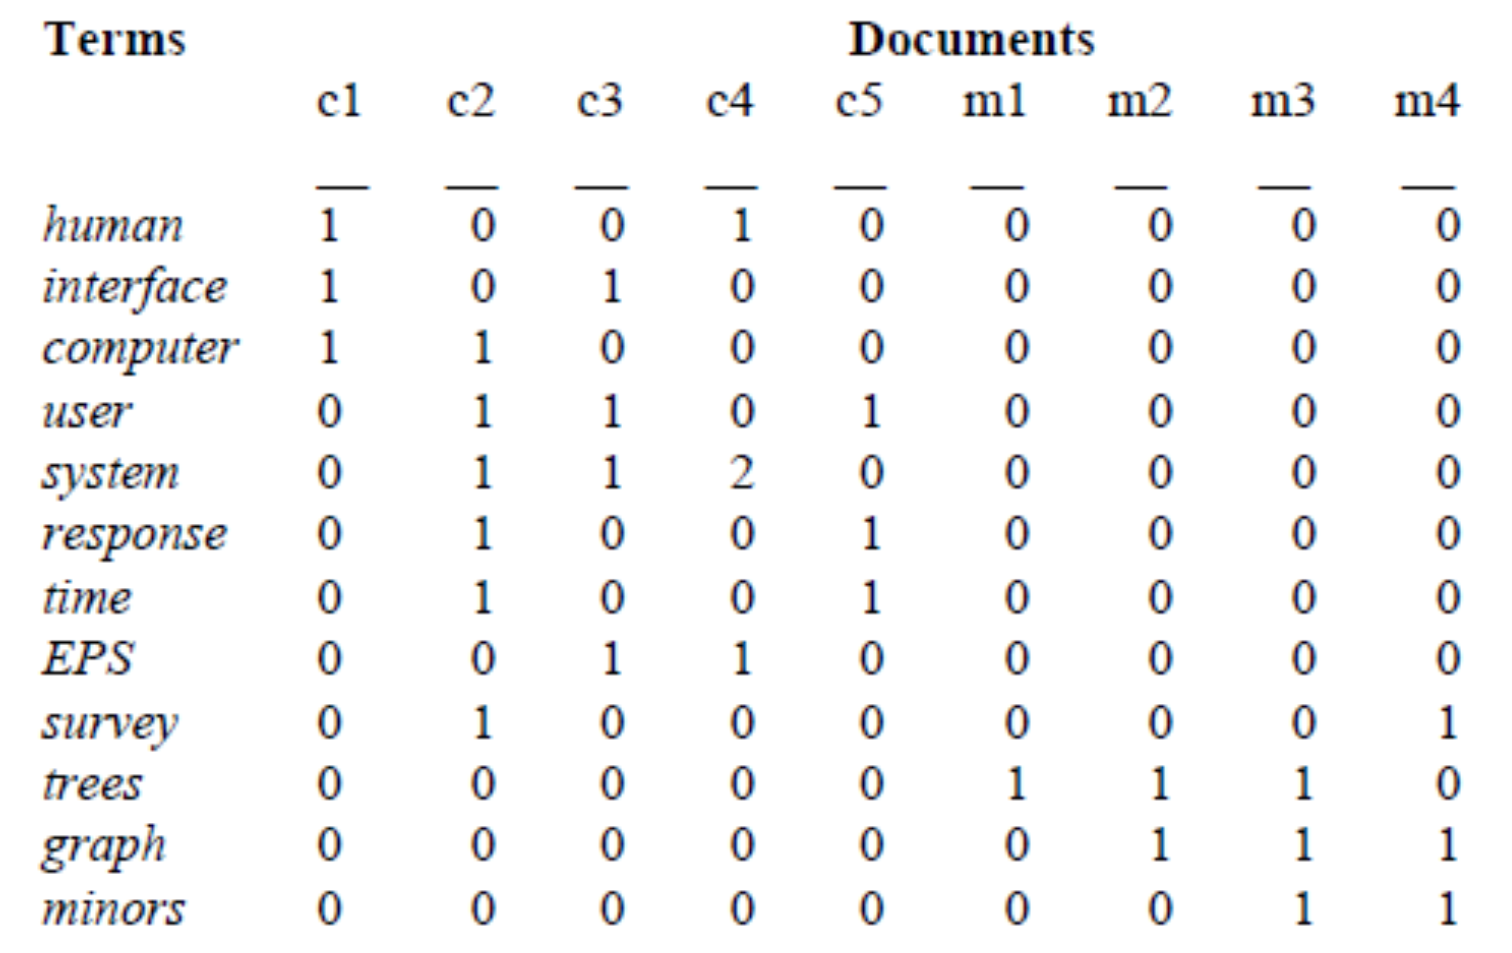
\includegraphics[width=0.4\textwidth]{pic/6.png}
%        \caption*{Original Document-Term Matrix}
%    \end{figure}
%    \begin{itemize}
%        \item Here is an example of a document-term matrix (Figure 1) where each cell represents the frequency of a term in a document.
%        \item LSI applies SVD to decompose this matrix, creating a lower-dimensional representation while retaining essential information.
%    \end{itemize}
%\end{frame}
%
%\begin{frame}{LSI Example: Reduced Representation with \( k=2 \)}
%    \begin{figure}
%        \centering
%        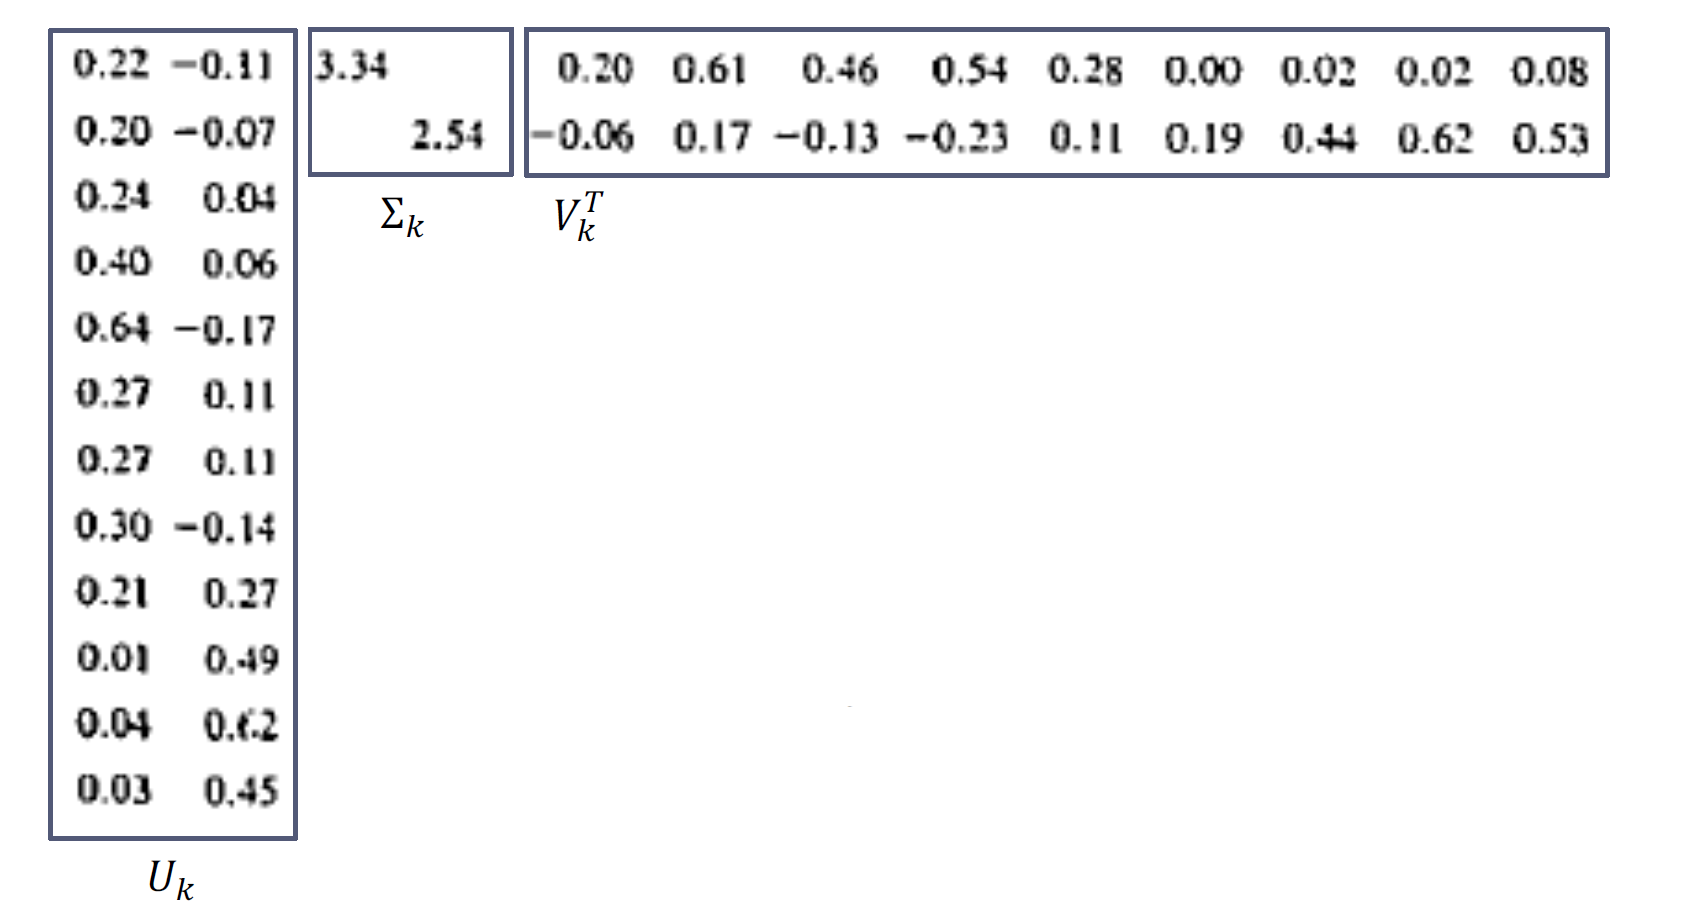
\includegraphics[width=0.35\textwidth]{pic/7.png}
%        \caption*{Decomposed Document-Term Matrix with \( k=2 \)}
%    \end{figure}
%    \begin{itemize}
%        \item After applying SVD, we retain only the top 2 singular values (Figure 2).
%        \item Similar terms and documents are now mapped close to each other in this reduced space, capturing underlying semantic relationships.
%        \item This transformation helps to reveal latent semantic structures that are less apparent in the original matrix.
%    \end{itemize}
%\end{frame}
%
%\begin{frame}{Dimensionality Reduction with LSI}
%    \begin{itemize}
%        \item In the reduced space, documents and terms that are similar are located closer together.
%        \item This helps in capturing latent semantic structures, which are not explicitly present in the original high-dimensional space.
%    \end{itemize}
%    \begin{figure}
%        \centering
%        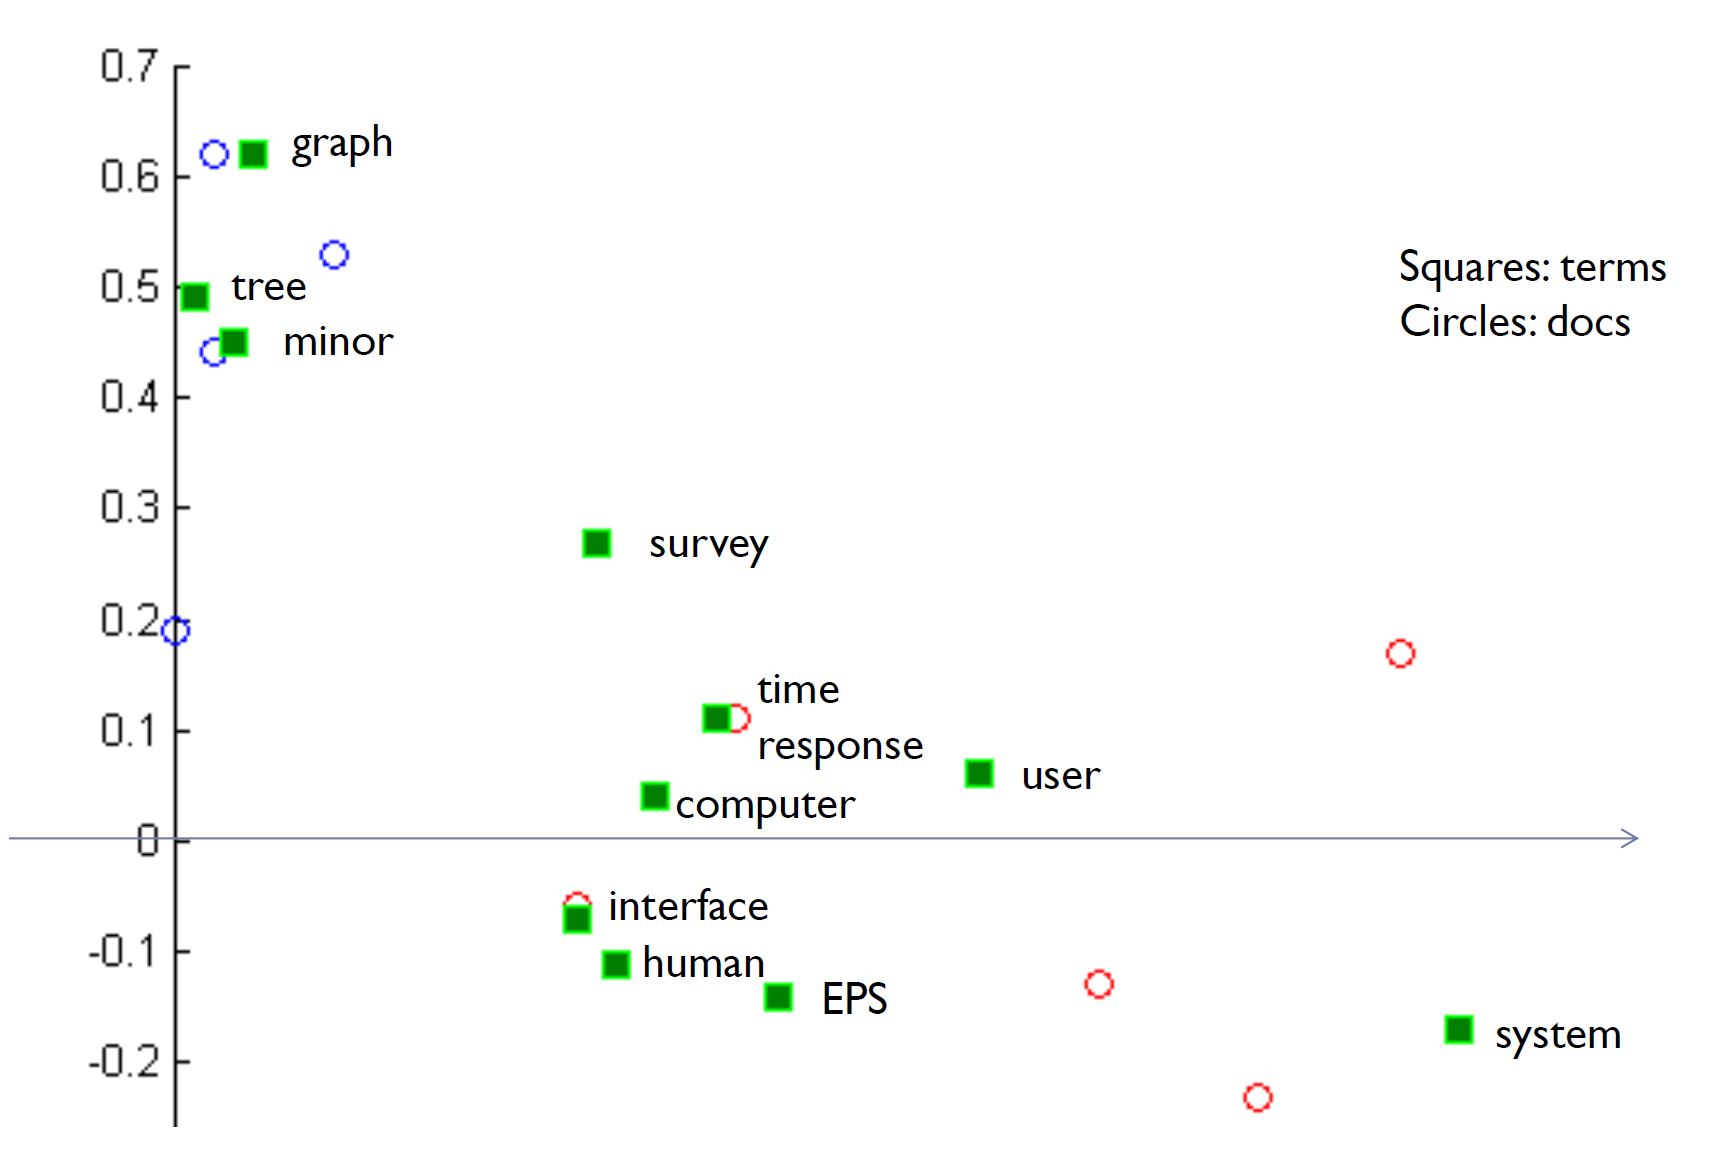
\includegraphics[width=0.4\textwidth]{pic/2.png}
%        \caption*{Visualization of reduced dimensional space}
%    \end{figure}
%\end{frame}
%
%\begin{frame}{LSI Example}
%    \begin{figure}
%        \centering
%        
\includegraphics[width=0.5\textwidth]{pic/1.png}
%        \caption*{Example of LSI on a term-document matrix}
%    \end{figure}
%    \begin{itemize}
%        \item After applying SVD, similar terms are mapped close to each other in the reduced space.
%        \item This helps capture synonymy and semantic relatedness between terms.
%    \end{itemize}
%\end{frame}
%
%\begin{frame}{Benefits of LSI}
%    \begin{itemize}
%        \item \textbf{Noise Reduction}: LSI removes the noise caused by variations in word usage by mapping similar words to the same dimension.
%        \item \textbf{Synonymy}: It helps address synonymy by grouping semantically related words together in the reduced space.
%        \item \textbf{Efficiency}: Reducing the dimensionality speeds up information retrieval processes and improves the performance of downstream tasks.
%    \end{itemize}
%\end{frame}
%
%\begin{frame}{Limitations of LSI}
%    \begin{itemize}
%        \item \textbf{Computational Cost}: The SVD operation can be computationally expensive, especially for large datasets.
%        \item \textbf{New Words}: It is hard to incorporate new words or documents once the model is trained.
%        \item \textbf{Order Ignorance}: LSI does not consider the order of words in documents, which may lead to the loss of important context.
%    \end{itemize}
%\end{frame}
%
%





\section{Word2Vec}

\begin{frame}{Why Learn Word Vectors?} 
	
	\begin{itemize} \item To process text data, we need to represent words in a form that a machine can understand—numerical vectors. \item Word2Vec uses a neural network to learn word embeddings that capture semantic similarities. \item These embeddings allow words with similar meanings to be represented by vectors close to each other in a high-dimensional space. 
	\end{itemize} 
\end{frame}

\begin{frame}{Word2Vec as a Neural Network}
	 \begin{itemize} \item Word2Vec operates like a shallow neural network, with an input, hidden, and output layer. \item It takes in a target word and learns to predict either the surrounding context words or the target word from a set of context words. \item Through training, the network adjusts weights to create meaningful vector representations of words. 
	 \end{itemize} 
\end{frame}


\begin{frame}{Word2Vec as a Neural Network}
	\begin{figure}
		\centering
		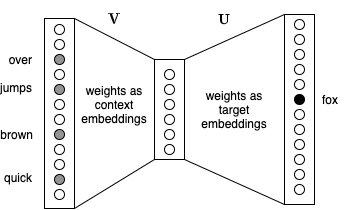
\includegraphics[width=0.6\textwidth]{pic/word2vec_nn.png}
		\caption*{Word2Vec as a two layer neural network}
	\end{figure}
	\vspace{0.4cm}
	\hspace{-1.0cm}
	{\tiny \textcolor{gray}{Figure adapted from medium.com/@manansuri/a-dummys-guide-to-word2vec-456444f3c673}}
\end{frame}

\begin{frame}{Expected Outcome of Word2Vec}
	\begin{itemize}
		\item Word2Vec aims to create a vector space where words with similar meanings or contexts are located close to each other.
		\item \textbf{Expected Result:} Semantically related words—such as “king” and “queen” or “dog” and “puppy”—should have similar vector representations.
		\item This proximity allows for various NLP tasks, such as:
		\begin{itemize}
			\item \textbf{Synonym detection:} Identifying words with similar meanings.
			\item \textbf{Analogy tasks:} Solving analogies by vector arithmetic (e.g., “king” - “man” + “woman” ≈ “queen”).
			\item \textbf{Clustering of concepts:} Grouping related concepts together in the embedding space.
		\end{itemize}
		\item By representing words in this way, Word2Vec enables models to make use of semantic relationships between words.
	\end{itemize}
\end{frame}



\begin{frame}{Expected Outcome of Word2Vec}
	\begin{figure}
		\centering
		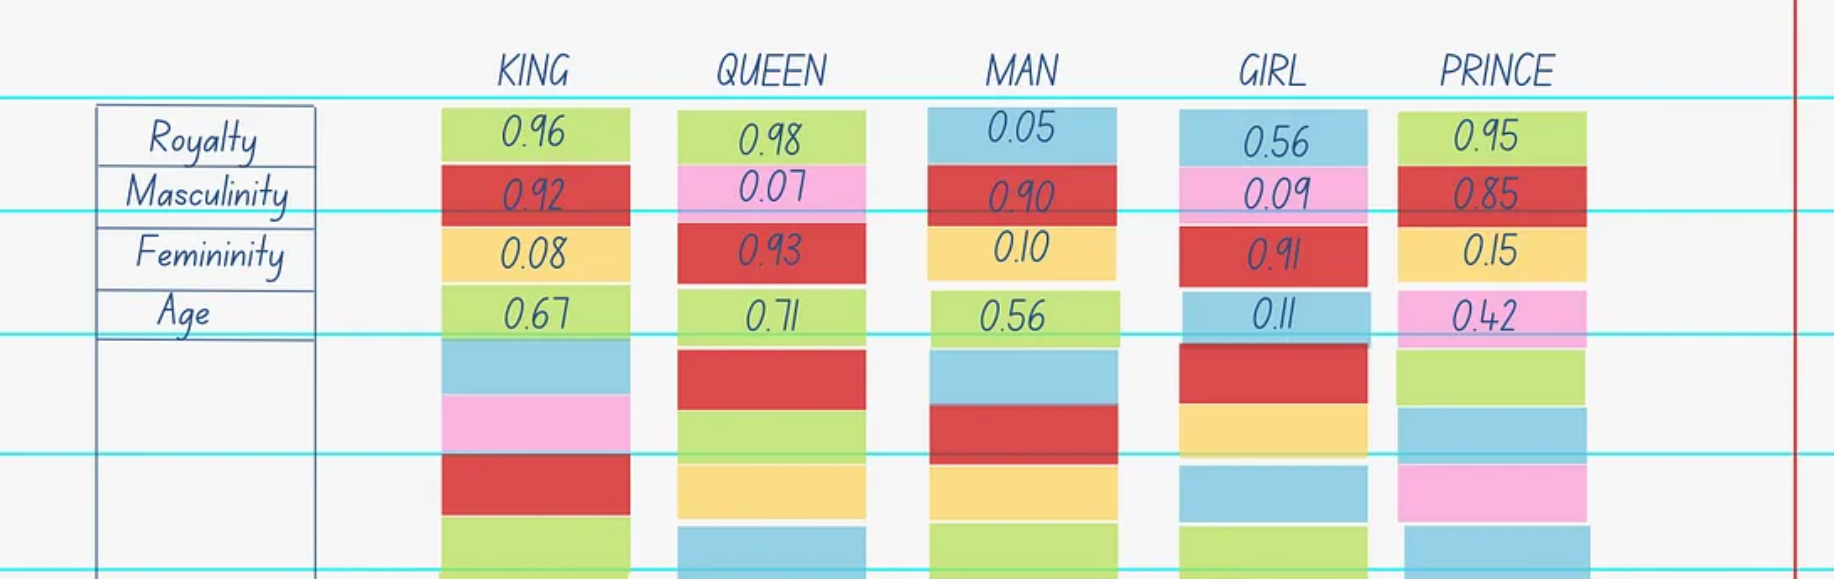
\includegraphics[width=1.0\textwidth]{pic/word2vec_expected.png}
		\caption*{Hypothetical features to understand word embeddings}
	\end{figure}
	\vspace{0.6cm}
	\hspace{-1.0cm}
	{\tiny \textcolor{gray}{Figure adapted from medium.com/@manansuri/a-dummys-guide-to-word2vec-456444f3c673}}
\end{frame}


%
%\begin{frame}{What is Word2Vec?}
%    \begin{itemize}
%        \item Word2Vec is a framework for learning word embeddings by predicting the surrounding words in a context window.
%        \item It represents words as continuous vectors in a dense vector space, where semantically similar words are close to each other.
%        \item Word2Vec captures the context of a word by using its surrounding words to represent its meaning.
%    \end{itemize}
%\end{frame}

\begin{frame}{Word2Vec: Contextual Word Representation}
    \begin{itemize}
        \item The core idea is based on distributional semantics: "You shall know a word by the company it keeps."
        \item Word2Vec uses two main algorithms for learning word vectors:
        \begin{itemize}
            \item Continuous Bag of Words (CBOW)
            \item Skip-gram Model
        \end{itemize}
    \end{itemize}
\end{frame}

\subsection{Continuous Bag of Words (CBOW)}

\begin{frame}{CBOW: How It Works}
    \begin{itemize}
        \item CBOW predicts the target word using the context (surrounding words) in a fixed window.
        \item For each word in the corpus, CBOW takes a set of context words and predicts the center word.
        \item Example: Given the context words \{“the”, “brown”, “fox”, “over”\}, CBOW predicts the center word “jumps.”
        \item CBOW tends to perform better on smaller datasets and is computationally more efficient.
    \end{itemize}
\end{frame}

\subsection{Skip-gram Model}

\begin{frame}{Skip-gram: How It Works}
    \begin{itemize}
        \item Skip-gram is the reverse of CBOW. It predicts the surrounding context words given a target word.
        \item For each word \(w_t\), the model predicts the words in the window of size \(m\) around it (e.g., words \(w_{t-2}, w_{t-1}, w_{t+1}, w_{t+2}\)).
        \item Example: If the center word is “jumps,” Skip-gram predicts the context words “the,” “brown,” “fox,” and “over.”
        \item Skip-gram is better suited for larger datasets and can capture rare words more effectively.
    \end{itemize}
\end{frame}


\begin{frame}{Skip-gram Example}
    \begin{figure}
        \centering
        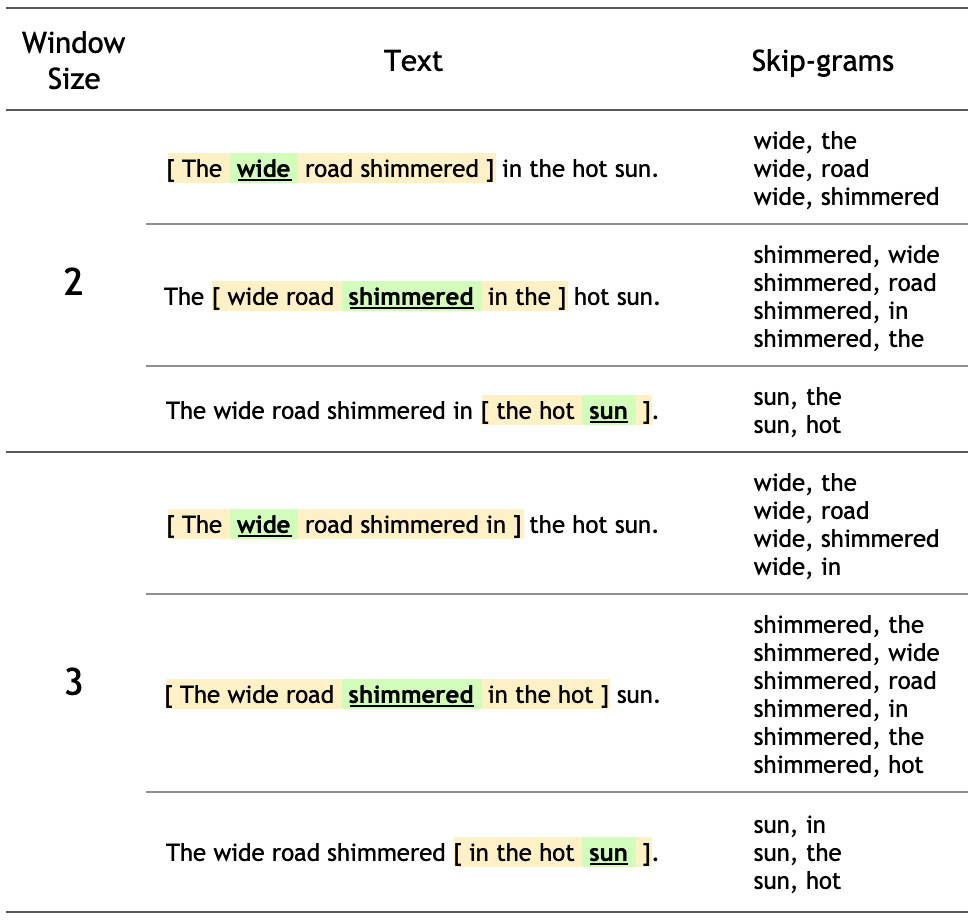
\includegraphics[width=0.4\textwidth]{pic/10.png}
        \caption*{Different window sizes and samples drawn from context words and their target}
    \end{figure}
    \vspace{0.1cm}
    \hspace{-1.0cm}
    {\tiny \textcolor{gray}{Figure adapted from tensorflow.org/text/tutorials/word2vec}}
\end{frame}



\begin{frame}{Skip-gram: Objective Function}
    \begin{itemize}
        \item The objective of Skip-gram is to maximize the likelihood of predicting context words \(w_o\) given a center word \(w_c\).
        \item The probability of a context word \(w_o\) given a center word \(w_c\) is defined as:
        \[
        P(w_o | w_c) = \frac{\exp(v_{w_o} \cdot v_{w_c})}{\sum_{w \in V} \exp(v_w \cdot v_{w_c})}
        \]
        \item \(v_{w_o}\) and \(v_{w_c}\) are the word vectors for the context and center words, respectively.
    \end{itemize}
\end{frame}

\begin{frame}{Skip-gram: Loss Function}
    \begin{itemize}
        \item The goal is to minimize the negative log-likelihood over the entire training corpus:
        \[
        J(\theta) = -\frac{1}{T} \sum_{t=1}^{T} \sum_{-m \leq j \leq m, j \neq 0} \log P(w_{t+j} | w_t)
        \]
        \item Here, \(T\) is the total number of words, and \(m\) is the window size.
        \item Skip-gram adjusts the word vectors to maximize the probability of observing the context words around the center word.
    \end{itemize}
\end{frame}


\begin{frame}{Skip-gram: Gradient Calculation}
    \begin{itemize}
        \item To update the word vectors during training, we calculate the gradient of the objective function.
        \item The gradient with respect to the word vector \(v_I\) is:
        \[
        \frac{\partial \log P(w_o | w_I)}{\partial v_I} = u_o - \sum_x P(w_x | w_I) u_x
        \]
    \end{itemize}
\end{frame}



\begin{frame}{Skip-gram: Gradient Calculation}
    \begin{itemize}
        \item The detailed steps for the gradient calculation are:
        \[
        \frac{\partial \log P(w_o | w_I)}{\partial v_I} = \frac{\partial}{\partial v_I} \log \frac{e^{u_o^T v_I}}{\sum_x e^{u_x^T v_I}}
        \]
        \[
        = \frac{\partial}{\partial v_I} \left( \log e^{u_o^T v_I} - \log \sum_x e^{u_x^T v_I} \right)
        \]
        \[
        = u_o - \frac{1}{\sum_x e^{u_x^T v_I}} \sum_x u_x e^{u_x^T v_I}
        \]
        \[
        = u_o - \sum_x P(w_x | w_I) u_x
        \]
        \item The update rule for \(v_{w_c}\) is:
        \[
        v_{w_c} \leftarrow v_{w_c} + \eta \left( v_{w_o} - \sum_{w \in V} P(w | w_c) v_w \right)
        \]
        \item Here, \(\eta\) is the learning rate.
    \end{itemize}
\end{frame}


\begin{frame}{Skip-gram Example}
    \begin{itemize}
        \item Consider the sentence: "The quick brown fox jumps over the lazy dog."
        \item If the center word is "jumps", the model predicts context words such as "quick", "brown", "fox", "over", and "the".
        \item The model iteratively adjusts word vectors to predict these context words, learning a meaningful representation for "jumps."
    \end{itemize}
\end{frame}



\begin{frame}{Skip-Gram Pseudocode}
	\begin{algorithm}[H]
		\caption{Skip-Gram Model}
		\begin{algorithmic}
			\fontsize{6pt}{7.2}\selectfont
			\Require Corpus $D$, window size $w$, embedding dimension $d$, learning rate $\alpha$, number of epochs $n$
			\State Initialize word embeddings $W$ and $C$ randomly, where $W$ maps words to embeddings and $C$ maps context words to embeddings
			
			\For{each epoch in $1$ to $n$}
			\For{each sentence $S$ in $D$}
			\For{each word $w_t$ in $S$}
			\State Extract context words within window size $w$ around $w_t$
			\For{each context word $c$ of $w_t$}
			\State Compute dot product $\text{score} = W(w_t) \cdot C(c)$
			\State Compute probability $P(c|w_t)$ using softmax: 
			\[
			P(c|w_t) = \frac{\exp(\text{score})}{\sum_{c' \in \text{vocab}} \exp(W(w_t) \cdot C(c'))}
			\]
			\State Calculate loss $L = -\log P(c|w_t)$
			\State Update $W(w_t)$ and $C(c)$ using gradient descent with learning rate \(\eta\)
			\EndFor
			\EndFor
			\EndFor
			\EndFor
			\State \Return Word embeddings $W$
		\end{algorithmic}
	\end{algorithm}
\end{frame}




\begin{frame}{CBOW vs. Skip-gram}
    \begin{figure}
        \centering
        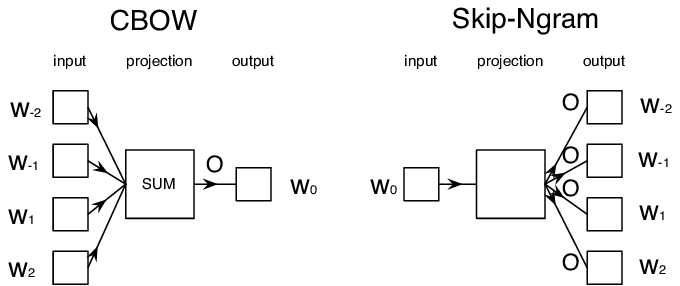
\includegraphics[width=0.8\textwidth]{pic/skip_vs_cbow.png}
        \caption*{Difference between CBOW and Skip-gram}
    \end{figure}
    \vspace{0.6cm}
    \hspace{-1.0cm}
    {\tiny \textcolor{gray}{Figure adapted from researchgate.net/figure/llustration-of-the-Skip-gram-and-Continuous-Bag-of-Word-CBOW-models_fig1_281812760}}
\end{frame}


\begin{frame}{CBOW vs. Skip-gram}
	\begin{itemize}
		\item CBOW and Skip-gram are the two primary architectures for Word2Vec.
		\item \textbf{CBOW} predicts a target word given its surrounding context, making it efficient and effective for smaller datasets.
		\item \textbf{Skip-gram}, on the other hand, predicts the surrounding words for a given target word. It is well-suited for larger datasets and can handle rare words more effectively.
		\item In essence, the Skip-gram model captures more detailed word relationships and is robust in large vocabularies.
	\end{itemize}
\end{frame}


\begin{frame}{Skip-gram as a Neural Network}
    \begin{itemize}
        \item The Skip-gram model functions as a two-layer neural network. 
        \item The input layer consists of a one-hot encoded target word vector, while the hidden layer is a dense embedding layer that learns the word representation.
        \item The output layer uses softmax to calculate the probability distribution over all words in the vocabulary, given the context.
        \item The Skip-gram model iteratively adjusts weights to maximize the likelihood of predicting the correct context words, ultimately learning meaningful word embeddings.
    \end{itemize}
\end{frame}


\begin{frame}{Skip-gram as a Neural Network}
	\begin{figure}
		\centering
		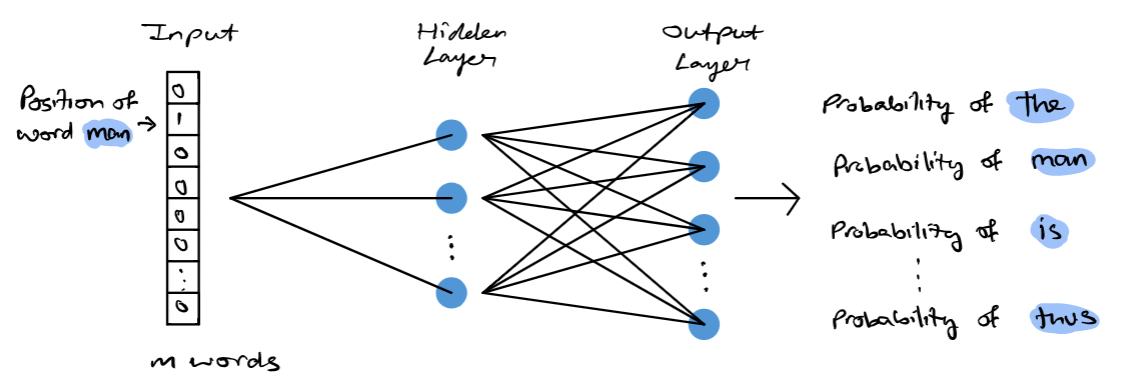
\includegraphics[width=0.8\textwidth]{pic/skip_nn.png}
		\caption*{Skip-gram Model as Neural Network}
	\end{figure}
	\vspace{1.0cm}
	\hspace{-1.0cm}
	{\tiny \textcolor{gray}{Figure adapted from towardsdatascience.com/word2vec-explained-49c52b4ccb71}}
\end{frame}

\begin{frame}{Why Do We Need Negative Sampling?}
    \begin{itemize}
        \item The softmax function normalizes over all words in the vocabulary \(V\), which can be very large (millions of words).
        \item This makes the calculation of \(\sum_{w \in V} \exp(v_w \cdot v_{w_c})\) expensive, as it requires summing over all words in the vocabulary.
        \item \textbf{Solution}: Use \textbf{Negative Sampling} to only update a few randomly chosen "negative" words instead of the entire vocabulary.
    \end{itemize}
\end{frame}

\begin{frame}{Skip-gram: Negative Sampling}
    \begin{itemize}
        \item In \textbf{negative sampling}, we sample a few "negative" words that do not appear in the context of the target word.
        \item For each positive pair (center word and context word), we sample \(k\) negative words that are not in the context.
        \item Instead of maximizing the probability of all words in the vocabulary, we only maximize the probability of the context words and minimize the probability of the sampled negative words.
        \item Example: If the center word is "cat", and the context word is "cute", we sample negative words like "computer", "sky", and "table" to minimize their probability in this context.
    \end{itemize}
\end{frame}

\begin{frame}{Skip-gram: Negative Sampling}
	\begin{figure}
		\centering
		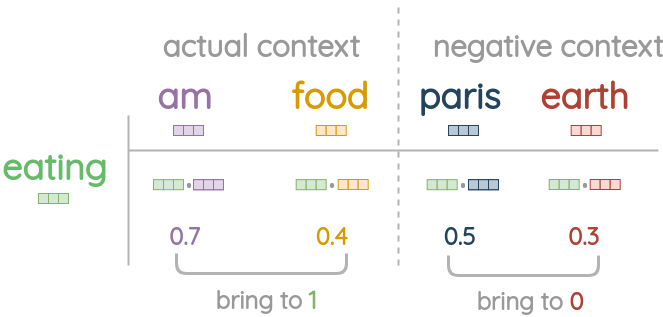
\includegraphics[width=0.8\textwidth]{pic/skip_negative.png}
		\caption*{Negative sampling}
	\end{figure}
	\vspace{0.6cm}
	\hspace{-1.0cm}
	{\tiny \textcolor{gray}{Figure adapted from jalammar.github.io/illustrated-word2vec/}}
\end{frame}


\begin{frame}{Why Skip-gram?}
    \begin{itemize}
        \item Skip-gram is preferred for large datasets because it handles rare words more effectively than CBOW.
        \item It captures detailed information about the surrounding words, leading to better word representations in the vector space.
        \item Word2Vec embeddings from Skip-gram have been widely adopted in various NLP tasks such as machine translation, sentiment analysis, and document classification.
    \end{itemize}
\end{frame}

\subsection{Word Embedding Visualization}

\begin{frame}{Visualizing Words in 2D}
    \begin{itemize}
        \item After training the model, words are mapped into a high-dimensional vector space.
        \item Using techniques like PCA or t-SNE, these vectors can be reduced to 2D for visualization, where similar words appear closer together.
    \end{itemize}
\end{frame}

\begin{frame}{Visualizing Words in 2D}
	\begin{figure}
		\centering
		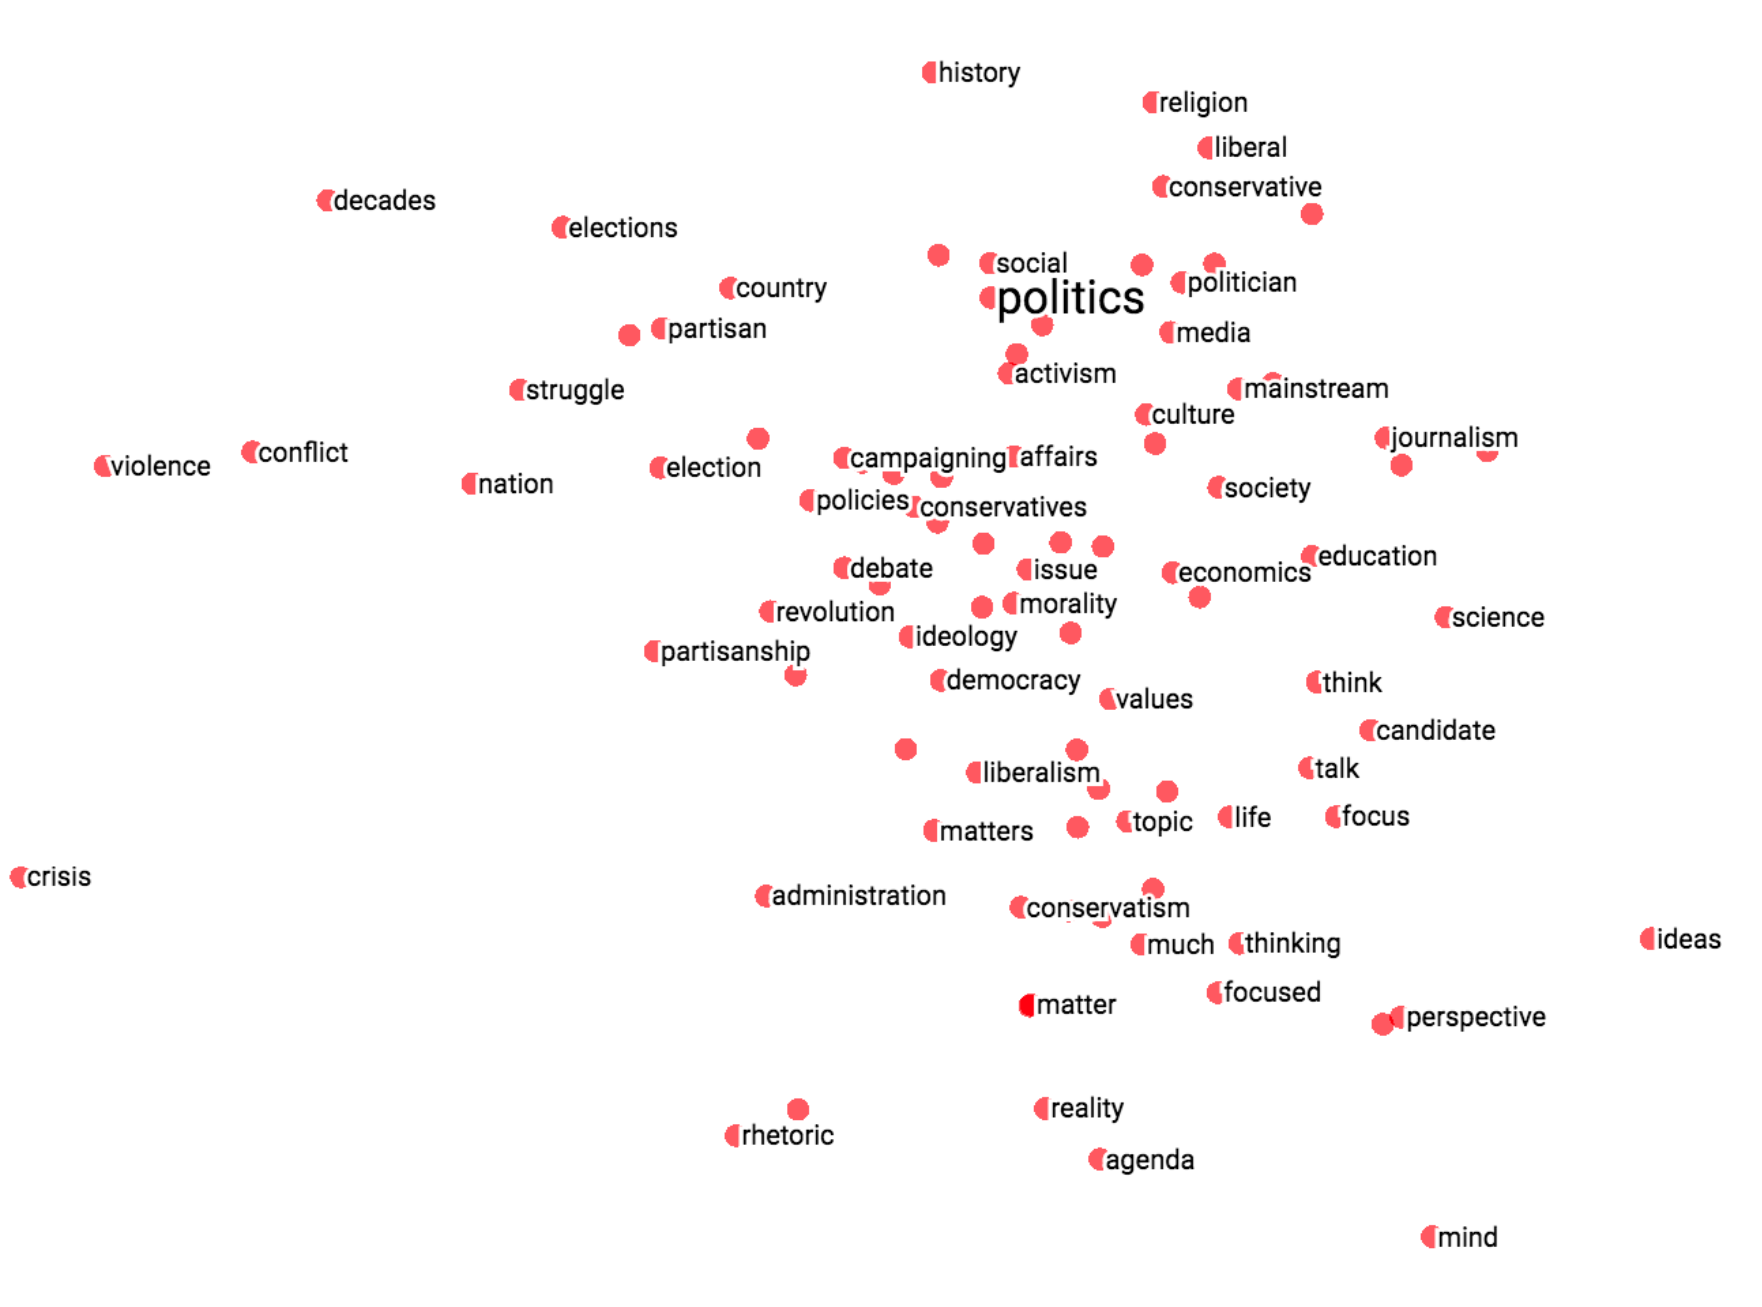
\includegraphics[width=0.6\textwidth]{pic/3.png}
		\caption*{Words represented in a 2D space after dimensionality reduction}
	\end{figure}
\end{frame}

\subsection{Word Analogy}

\begin{frame}{Word Analogy: Vector Arithmetic in Word2Vec}
    \begin{itemize}
        \item Word2Vec embeddings can solve analogy tasks by performing vector arithmetic.
        \item The analogy task takes the form:
        \[
        \text{king} - \text{man} + \text{woman} \approx \text{queen}
        \]
        \item The analogy is solved by finding the word vector closest to \( \mathbf{v}_{king} - \mathbf{v}_{man} + \mathbf{v}_{woman} \).
    \end{itemize}
\end{frame}

\begin{frame}{Word Analogy Example}
    \begin{itemize}
        \item Example:
        \[
        \text{king}[0.30, 0.70] - \text{man}[0.20, 0.20] + \text{woman}[0.60, 0.30] \approx \text{queen}[0.70, 0.80]
        \]
        \item This means the vector difference between "king" and "man" is similar to the difference between "queen" and "woman."
    \end{itemize}
\end{frame}


\begin{frame}{Word Analogy Example}
	\begin{figure}
		\centering
		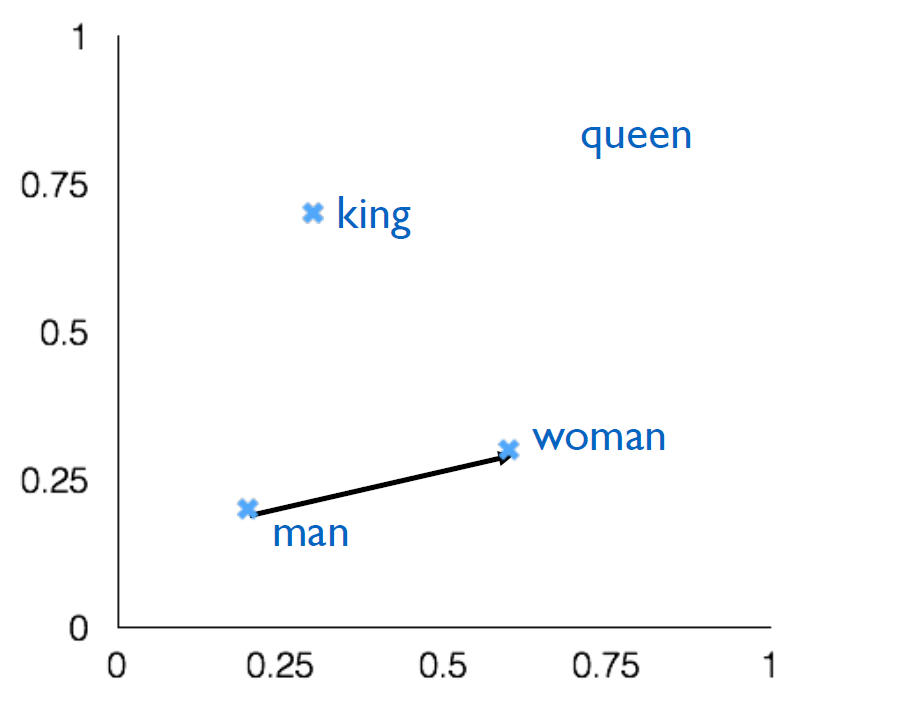
\includegraphics[width=0.5\textwidth]{pic/4.png}
		\caption*{Word analogy example}
	\end{figure}
\end{frame}

\begin{frame}{Word Analogy Formula}
    \begin{itemize}
        \item The formal formula for solving word analogies is:
        \[
        d = \arg\max_i \frac{(x_b - x_a + x_c)^T x_i}{\|x_b - x_a + x_c\|}
        \]
        \item This finds the word \(x_i\) whose vector is closest to the result of the vector arithmetic.
    \end{itemize}
\end{frame}








\section{References}



\begin{frame}[allowframebreaks]
    \bibliography{ref}
    \bibliographystyle{ieeetr}
    \nocite{*}
\end{frame}

\end{document}